\subsubsection{Diseño de VMware vCenter Server}
El componente VMware vCenter Server es el punto de acceso y de control de todas las máquinas virtuales localizados en los hosts ESXi que forman parte de su dominio. En el entorno desplegado se utiliza una instancia de VMware vCenter Server para controlar el \textit{management domain}, se denomina \textit{vcenter-mgmt}. Esta instancia de vCenter Server contiene un dominio que con un cluster vSphere formado por los cuatro hosts ESXi desplegados por VLC, estos se denominan respectivamente \textit{esxi-1}, \textit{esxi-2}, \textit{esxi-3} y \textit{esxi-4}. En vCenter Server se gestionan los recursos de las VMs de cada componente, se monitorizan los recursos, permite la creación y asignación de roles, permisos y usuarios, aisla las redes que usan los recursos que controla de otras instancias de vCenter Server, permite gestionar los grupos de discos de almacenamiento de cada host ESXi que forman el \textit{datastore} de VMware vSAN, administrar las redes a las que se conecta cada componente, en definitiva, VMware vCenter Server es el punto desde el cual se controlan los recursos que utiliza cada componente. Además, incluye el componente PSC que controla el dominio de autenticación de VMware vSphere SSO Domain denominado \textit{local}. Desde vCenter Server también se controlan las características de alta disponibilidad y recuperación ante fallos de VMware vSphere como se verá a continuación. El acceso a vCenter Server se hace a través del componente web vSphere Client.
\begin{figure}[h]
  \centering
  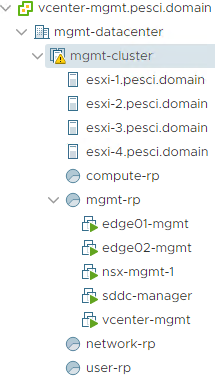
\includegraphics[width=0.2\textwidth]{imaxes/pruebaconcepto/clusterVCenterServer.png}
  \caption{Dominio y cluster vSphere del \textit{management domain}.}
  \label{fig:cluster-vCenter-Server}
\end{figure}
\FloatBarrier
En la imagen anterior se muestra el dominio (\textit{vcenter-mgmt.pesci.domain}) de la instancia de vCenter Server y el cluster vSphere (\textit{mgmt-cluster}) donde se alojan los componentes del \textit{management domain}. Incluye cuatro hosts ESXi y cuatro \textit{resource pools}, uno de ellos contiene las VMs de los componentes dedicados a este \textit{management domain}.
%  Con vCenter Server se simplifica la escalabilidad del SDDC, la gestión de actualizaciones para los componentes es más sencilla, permite determinar roles específicos y responsabilidades y permite aislar las redes de otras instancias de vCenter Server. Además, para gestionar vSpehere SSO Domain, VMware vCenter Server contiene embebido el componente PSC con todos los servicios necesarios. 
%  En caso de que existan varios \textit{Workload Domain} se puede habilitar el modo \textit{Enhanced Linked Mode} para poder gestionar todas las instancias de vCenter Server de forma centralizada desde un único vSphere Client.
% Por lo anterior, en el \textit{management domain} se despliega una instancia de VMware vCenter Server que incluye un cluster de VMware vSphere.

\begin{subsubsection}{Diseño almacenamiento VMware vSAN}
  El almacenamiento del \textit{management domain} desplegado, está implementado con VMwware vSAN. Los cuatro hosts ESXi contienen cuatro grupos de discos cada uno con configuración All-Flash. Como hay cuatro hosts participantes, soporta el fallo de un host lo cual permite dejar hosts fuera de servicio para tareas de mantenimiento. Esto es posible gracias a que con FTT (\textit{Failures-To-Tolerate}) igual a 1 se mantiene la redundancia de los datos almacenados en el \textit{datasotore}, en uno de los hosts. Cada grupo de discos cuenta con cuatro discos uno de ellos para caché, 16 discos en total. Para hacer disponible este servicio de almacenamiento, todos los hosts deben estar conectados a la subred generada para VMware vSAN y utilizar una VLAN para separar su tráfico.
\end{subsubsection}
    
\begin{subsubsection}{Diseño cluster VMware vSphere}
Dentro de un \textit{workload domain} pueden existir varios clusters vSphere con diferentes características según su finalidad. Los hosts ESXi que lo forman pueden ser de diferentes tamaños teniendo en cuenta que se pueden usar menos hosts ESXi de mayor capacidad o más hosts con menores prestaciones, el coste de cada host ESXi, el uso que se le va a dar al cluster y las características máximas y mínimas del cluster vSphere. Debido a la limitada cantidad de recursos que ofrece el host físico donde se realiza el despliegue, para el \textit{management domain} se utiliza un único cluster vSphere con de 4 hosts de los cuales se reserva un host para proveer redundancia. Todos los hosts ESXi cuenta con 64GB de memoria RAM menos uno que tiene 32 GB, y 19.9GHz de CPU. Dentro del cluster hay que configurar los servicios vSphere HA y vSphere DRS para proteger los componentes del SDDC. La configuración que se establece en el \textit{management domain} es la siguiente:
% En caso de que el \textit{management domain} esté extendido en dos AZ entonces se requieren 4 hosts en cada AZ para proporcionar redundancia y disponibilidad en caso de caída de una de las AZ.

\begin{itemize}
    \item \textbf{vSphere High Availability}: en este servicio la propiedad \textit{Admission Control Policy} permite establecer la cantidad de recursos reservados en caso de fallo y como se establece el cálculo de esos recursos. En el \textit{management domain} se configura para el fallo de al menos un host y reserva de recursos según un porcentaje, reservando así el 25\% de la CPU y el 30\% de la memoria RAM ya que funciona mejor cuando las VM usan mucha CPU y memoria. La otra propiedad que se debe habilitar para el correcto funcionamiento del servicio es \textit{VM and Application Monitoring}, que se encarga de reiniciar las VM en caso de caída.
    % que puede ser según el número hosts que pueden fallar en el cluster, según un porcentaje de reserva de rescursos o especificando el host donde se recolocan las VM del host caído.  RAM.  
    \item \textbf{vSphere DRS}: este servicio permite migrar VMs de un host ESXi a otro dentro del mismo cluster vSphere para equilibrar la carga de trabajo y mantener las VMs activas en caso de caída de alguno de los hosts. Se activa usando la opción por defecto \textit{Fully Automated} ya que aporta el mejor balance entre consumo de recursos y migraciones de VM innecesarias. Adicionalmente también se pueden establecer reglas para determinar el orden de encendido de las VMs pertenecientes a un mismo grupo. 
    %En caso de que exista más de una AZ, se deben crear grupos de VM y de hosts de cada AZ para luego implementar reglas de afinidad para que las VM de una AZ no sean migradas a otra AZ ya que esto puede afectar al rendimiento de la VM. 
\end{itemize}
% En el modelo consolidado se debe crear un único cluster con un mínimo de cuatro hosts ESXi ya que uno de los hosts se utiliza para asegurar la disponibilidad del almacenamiento vSAN cuando hay algún host inactivo. Este modelo proporciona capacidad de un único fallo por cluster.
\end{subsubsection}
\subsubsection{Diseño de red para el cluster vSphere}
Si bien en VMware Cloud Foundation existe VMware NSX-T, un componente dedicado únicamente a la administración de la red del SDDC, es desde VMware vSphere dónde se encuentran los elementos para establecer redes que separen cada tipo de tráfico de los componentes del SDDC. Estas redes se configuran en base a los siguientes aspectos:
\begin{itemize}
    \item Separar el tráfico de cada servicio para mejorar la eficiencia de la red y la seguridad. Así se puede ajustar las características de cada red, como el ancho de banda o la latencia, a las necesidades de cada servicio.
    \item Utilizar un único vSphere Distributed Switch por cluster donde se añade un \textit{port group} por cada servicio.
    % \item Mejorar el rendimiento usando NICs de tipo VMXNET3 en las máquinas virtuales.
    \item Las NICs físicas de cada host ESXi conectados a un mismo vSphere Distributed Switch están conectadas también a la misma red física.
    % \item Aquellas redes que se dedican a servicios de la infraestructura deben estar configuradas con puertos tipo \textit{vmkernel}.
\end{itemize}
Para el \textit{management domain} del SDDC se crea un único vSphere Distributed Switch llamado \textit{sddc-vds01} con la siguiente configuración:
\begin{itemize}
    
    \item Se establece un MTU igual 9000 Bytes para permitir el tráfico de \textit{jumbo frames} ya que son requeridos por algunos de los servicios.
    
    \item Se habilita el servicio \textit{Network I/O} que permite establecer un nivel de prioridad a cada tipo de tráfico. Esto se realiza estableciendo limites de ancho de banda, políticas de balanceo de carga y reserva de recursos para un tipo de tráfico asociado a un servicio. Por cada tipo de tráfico hay cuatro aspectos que se pueden configurar que son \textit{Shares} (indica el \% de ancho de banda que se le da a un tipo de tráfico, el tipo de tráfico que tenga un mayor valor en \textit{Shares} tendrá más prioridad a la hora de usar los recursos), \textit{Reservation} (indica el valor de ancho de banda que se reserva para el tipo de tráfico) y \textit{Limit} (establece un valor máximo para el ancho de banda de un tipo de tráfico). En el \textit{management domain} los tipos de tráfico más relevantes que se deben configurar son los siguientes:
    \begin{itemize}
      \item \textit{Management Traffic}: el valor \textit{Shares} se establece al 50\% (\textit{Normal}) lo cual le da mayor prioridad que el resto de tipos. El resto de valores no se modifican.
      \item \textit{vSphere vMotion Traffic}: el valor \textit{Shares} se establece al 25\% (\textit{Low}) ya que durante el estado normal del entorno este tipo de tráfico no es muy importante. El resto de valores no se modifican.
      \item \textit{vSAN Traffic}: el valor \textit{Shares} se establece al 100\% (\textit{High}) para garantizar que este servicio recibe la cantidad de ancho de banda que necesita. El resto de valores no se modifican.
      \item \textit{Virtual Machine Traffic}: el valor \textit{Shares} se establece al 100\% (\textit{High}) para garantizar que las VMs siempre tienen acceso a la red ya que son una parte importante del SDDC. El resto de valores no se modifican.
    \end{itemize}
    
    \item Para detectar errores de compatibilidad entre la configuración del vSphere Distributed Switch y la red física se habilita el servicio \textit{Health Check}. Este se encarga de comprobar si la configuración de cada VLAN y MTU se adapta a la configuración de la capa física.
    
    \item Como puertos de salida \textit{Uplink} se configuran las interfaces físicas \textit{vmnic0} y \textit{vmnic1}. Como vDS es un componente distribuído, en cada host se usarán ambas interfaces de red como \textit{uplinks}.
    
\end{itemize}
En este vSpehere Distributed Switch para el Management Domain se configuran los siguientes \textit{port groups}, que son de tipo \textit{Distributed port group} y de tipo \textit{Uplink port group}. Además, el vDS está configurado sobre los cuatro hosts por lo tanto todos tienen acceso a todos los \textit{port groups}:
\begin{itemize}
       
        \item \textbf{Management port group}: es un \textit{Distributed port group} que comunica a todos los hosts ESXi entre si y transmite el tráfico entre los diferentes componentes de VMware Cloud Foundation, es decir, por este \textit{port group} circulan los comandos de configuración y gestión que los componentes del SDDC se envían entre ellos. Tiene el nombre \textit{sddc-vds01-mgmt}, a él se conectan las VMs \textit{vcenter-mgmt}, \textit{sddc-manager}, \textit{nsx-mgmt-1},\textit{edge01-mgmt} y \textit{edge02-mgmt}. Utiliza la subred con IP 10.0.0.0, máscara de red 255.255.255.0, VLAN 10 y MTU igual a 1500 Bytes. Esta red debe ser configurada también en la infraestructura física.
        
        \item \textbf{vMotion port group}: es un \textit{Distributed port group} que está dedicado al tráfico del componente vSphere vMotion para realizar las migraciones de máquinas virtuales de un host a otro. Tiene el nombre \textit{sddc-vds01-vmotion} y utiliza la subred con IP 10.0.4.0, máscara de red 255.255.255.0, VLAN 10 y MTU igual a 8940 Bytes.
        
        \item \textbf{vSAN port group}: es un \textit{Distributed port group} que está dedicado al servicio de almacenamiento VMware vSAN y por él los hosts acceden al almacenamiento del SDDC. Tiene el nombre \textit{sddc-vds01-vsan} y utiliza la subred con IP 10.0.8.0, máscara de red 255.255.255.0, VLAN 10 y MTU igual a 8940 Bytes.
        
        \item \textbf{Edge Uplink port group}: es un \textit{Distributed port group} dedicado a las conexiones del component NSX-T Edge que se dedica a dar acceso a determinados servicios y para proporcionar a otros \textit{workload domain} conexión con la red externa. Están gestionados por VMware NSX-T ya que dan servicio a sus componentes. En el entorno existen dos \textit{port groups} para proporcionar redundancia y alta dispobilidad, uno llamado \textit{sddc-edge-uplink01} cuyas instancias están configuradas bajo la red con IP 172.27.11.0 y con máscara de red 255.255.255.0, y otro llamado \textit{sddc-edge-uplink02} cuyas instancias están configuradas bajo la red con IP 172.27.12.0 y máscara de red 255.255.255.0. Ambos \textit{port groups} están configurados como VLAN Trunk (por ellos puede circular tráfico de cualquier VLAN) y tienen un MTU de 8940 Bytes. En ambos hay configuradas las dos VMs llamadas \textit{edge01-mgmt} y \textit{edge02-mgmt}. Estas dos redes también se deben configurar en la infraestructura física.
        
        \item \textbf{Uplink port group}: se trata de un \textit{Uplink port group} al que se le asignan las NICs físicas de cada host para establecer políticas sobre el tráfico que se dirige desde los hosts y VMs hacia fuera del vSphere Distributed Switch. Con el nombre \textit{sddc-vds01-DVUplinks-10}, en él están configuradas las dos NICs físicas de cada host, cada una en una interfaz \textit{uplink}.
        
\end{itemize}
\begin{figure}[h]
  \centering
  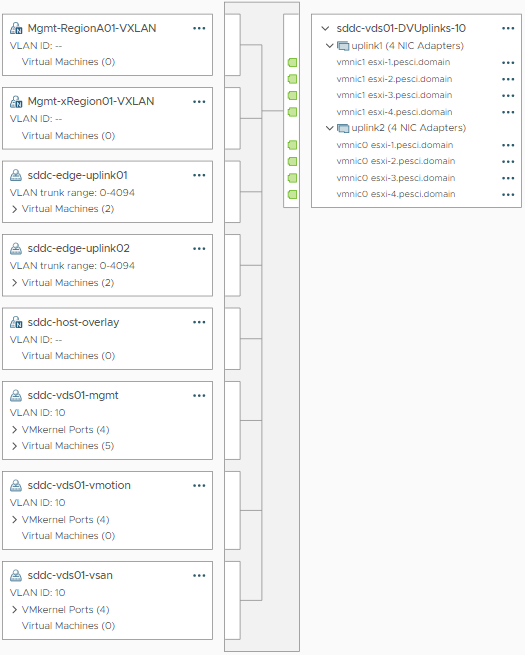
\includegraphics[width=0.4\textwidth]{imaxes/pruebaconcepto/distributedSwitchEntornoFinal.png}
  \caption{Contenido de vSphere Distributed Switch \textit{sddc-vds01}.}
  \label{fig:port-groups-vSwitch-vSphere}
\end{figure}
\FloatBarrier
En la imagen anterior se muestran todos los \textit{Distributed Port Groups} y \textit{Uplink port group} que se alojan en el vSphere Distributed Switch (\textit{sddc-vds01}) dedicado al \textit{management domain}. En el \textit{port group} \textit{sddc-vds01-DVUplinks-10} se muestra como cada interfaz \textit{uplink} se mapea con una interfaz física (vmnic) de cada host ESXi. Los \textit{port groups} \textit{mgmt-Region01A-VXLAN}, \textit{mgmt-xRegion01-VXLAN} y \textit{sddc-host-overlay} son generados y administrados por el componente VMware NSX-T como se explicará más adelante. Cada \textit{port group} informa de cuantas VMs y hosts ESXi tiene conectados.

La configuración que se aplica a cada \textit{Distributed port group} descrito anteriormente es la siguiente:
\begin{itemize}
  \item \textit{Port binding}: permite indidcar como se gestionan los puertos de un \textit{port group} cuando se añade o elimina una VM. Tiene dos opciones de configuración, la primera se denomina \textit{Static Port Binding} y su función consiste en asignar un puerto dentro del \textit{port group} a la VM que se conecta y solo se elimina cuando la VM es borrada. La segunda opción se denomina \textit{Ephemeral Port Binding} y consiste en que el puerto se asigna a la VM cuando esta se enciende y se elimina cuando se apaga o elimina. Para los \textit{port groups} \textit{sddc-vds01-vsan} y \textit{sddc-vds01-vmotion} se configura la opción \textit{Static Port Binding} ya que así se asegura que las VMs se conectan siempre al mismo puerto lo cual permite mantener datos históricos y hacer monitoreo a nivel de puerto. Para los \textit{port group} \textit{sddc-vds01-mgmt}, \textit{sddc-edge-uplink01} y \textit{sddc-edge-uplink02} se configura la opción \textit{Ephemeral Port Binding} ya que, como el tráfico que circula por ellos es el que gestiona todos los componentes del SDDC y dan acceso a otras redes externas, se elimina la dependencia con el estado de VMware vCenter Server permitiendo que la comunicación continúe aunque VMware vCenter Server no se encuentre operativo.

  \item \textit{Load Balancing}: indica como se distribuye el tráfico de salida de cada VM/host que se encuentran en el \textit{port group} entre las NICs físicas. Se selecciona \textit{Route based on physical NIC load}, es decir, el tráfico de una VM se transmite por una única NIC por lo que si esa NIC física está saturada, se asignará otra NIC física a la VM.
  
  \item \textit{Network failure detection}: esta opción permite establecer como debe determinar el \textit{port group} que alguna de las NICs físicas está fuera de servicio. Se selecciona \textit{Link status only} para que esto se determine según el estado que le transmite la NIC física, así se pueden detectar los fallos que ocurren en la red física.
  
  \item \textit{Notify switches}: se habilita para permitir a los host enviar \textit{frames} a los switches físicos para que estos conozcan la localización de las VM que están funcionando en cada host.
  
  \item \textit{Failback}: permite determinar como se reactiva una NIC cuando esta se recupera de un fallo. Se habilita para establecer que la NIC se marcará como activa inmediatamente después de que se haya recuperado. Esta opción se debería desactivar en caso de que el estado de la NIC sea inestable.
  
  \item \textit{Failover Order}: permite determinar que uplinks se deben utilizar, los que se seleccionan como \textit{active} son los que se utilizarán por defecto, los que se seleccionan como \textit{stand by} se usarán cuando los uplinks marcados como \textit{active} se encuentren desactivados. Se seleccionan las dos interfaces \textit{uplink} disponibles en el estado \textit{active}. Para el \textit{port group} \textit{sddc-edge-uplink01} se selecciona la interfaz \textit{uplink1} como activa y se deja sin usar la interfaz \textit{uplink2}, mientras que se configura de forma contraria en el \textit{port group} \textit{sddc-edge-uplink02}.
\end{itemize}